\documentclass{article}
\usepackage{graphicx} % Required for inserting images
\usepackage{enumitem}
\usepackage{amsmath}
\usepackage{float}

\title{ECCE148: Signal Processing Applications \\ \large
        Assignment 8: Digital High-pass Butterworth Filters}
\author{Andy Chen}
\date{May 2026}

\begin{document}

\maketitle

\section{Introduction}
The objective of this homework assignment is to construct a simple procedure for the design of \textit{digital high-pass Butterworth filters}. For simplicity and consistency, we use the \textit{bilinear transformation} method for frequency mapping between the analog and discrete domains.
\\
\\
The input to the procedure will be the standard design specifications of the digital high-pass filter. The design specifications are:
\begin{enumerate}[label=\alph*.,leftmargin=2cm, rightmargin=2cm]
    \item \textit{Pass-band Frequency}: \hfill \(\Omega_p=\pm\frac{5\pi}{6}\)
    \item \textit{Max. Pass-band Attenuation}: \hfill \(\alpha_{max}=0.5\text{ dB}\)
    \item \textit{Stop-band Frequency}: \hfill \(\Omega_s=\pm\frac{2\pi}{3}\)
    \item \textit{Min. Stop-band Attenuation}: \hfill \(\alpha_{min}=20\text{ dB}\)
\end{enumerate}

\section{Design Procedure}
We first identify the equivalent digital low-pass problem. The key insight is the spectral transformation \(z=-Z\), which maps \(H_{HP}(e^{j\Omega}) = H_{LP}(e^{j(\pi-\Omega)})\). Then, we pre-warp the digital low-pass edges to analog low-pass edges using the inverse bilinear formula: 
\[\omega=\beta\tan(\frac{\Omega}{2})\]
We compute the low-pass design order \(n\) and cutoff \(\omega_c\) from the Butterworth design equations, and construct the analog low-pass design \(H(s)\) from its Butterworth poles, scaled to \(\omega_c\). Then, we apply the bilinear transform:
\[
s=\beta\frac{z-1}{z+1}
\]
to get digital low-pass filter \(\hat{H}(z)\). After applying the transformation:
\[
z=-Z
\]
we will produce the digital high-pass filter \(H(z)\). Then, we verify the frequency response at \(\Omega_p\) and \(\Omega_s\).

\section{Analog Low-Pass Design Specifications}
Using the transformation:
\[
\Omega_{LP}=\pi-\Omega_{HP}
\]
we obtain the digital low-pass design specifications:
\[
\Omega_p=\frac{\pi}{6}
\]
\[
\Omega_s=\frac{\pi}{3}
\]
We then prewarp the frequencies with \(\beta=2\) using the transformation:
\[
\omega=\beta\tan\bigg(\frac{\Omega}{2}\bigg)
\]
Thus, obtaining the analog low-pass filter design specifications:
\begin{enumerate}[label=\alph*.,leftmargin=2cm, rightmargin=2cm]
    \item \textit{Pass-band Frequency}: \hfill \(\omega_p=\pm\ 0.536\) rad/s
    \item \textit{Max. Pass-band Attenuation}: \hfill \(\alpha_{max}=0.5\text{ dB}\)
    \item \textit{Stop-band Frequency}: \hfill \(\omega_s=\pm\ 1.155\) rad/s
    \item \textit{Min. Stop-band Attenuation}: \hfill \(\alpha_{min}=20\text{ dB}\)
\end{enumerate}

\section{Order and Cut-Off Frequency}
From the Butterworth order equation:
\[
n\geq\frac{\log_{10}(\frac{10^{\alpha_{min}/10}-1}{10^{\alpha_{max}/10}-1}\big)}{2\log_{10}(\omega_s/\omega_p)}
\]
we substitute in our analog low-pass filter design specifications and obtain:
\[
n\geq4.3631
\]
We round up to get our final order:
\[
n=5
\]
We determine the upper and lower bounds of the cut-off frequency:
\[
\frac{\omega_p}{(10^{\alpha_{max}/10}-1)^{\frac{1}{2n}}}\leq\omega_0\leq\frac{\omega_s}{(10^{\alpha_{min}/10}-1)^{\frac{1}{2n}}}
\]
\[
0.6614 \text{ rad/s }\leq\omega_0\leq0.7293 \text{ rad/s}
\]
We choose the lower bound of the cut-off frequency, yielding:
\[
\omega_0=0.6614\text{ rad/s}
\]

\section{Analog Low-Pass Filter \(H(s)\)}
We first identify the poles of the transfer function. Since \(n=5\) is odd, we have:
\[
s=\omega_0e^{j\frac{2k\pi}{10}}
\]
for \(k=0, 1, 2,\dots9\). We select the 5 poles on the left-half plane from the set of 10 (poles that will yield \(\theta=\frac{2k\pi}{10}\) between \(\frac{\pi}{2}\) and \(\frac{3\pi}{2}\)). We then formulate the transfer function:
\[
H(s)=\frac{\omega_0^n}{(s-s_1)(s-s_2)(s-s_3)(s-s_4)(s-s_5)}
\]
\[
H(s)=\frac{0.127}{(s-0.661e^{j\frac{2\pi}{10}3})(s-0.661e^{j\frac{2\pi}{10}4})((s+0.661)((s-0.661e^{j\frac{2\pi}{10}6})(s-0.661e^{j\frac{2\pi}{10}7})}
\]
Thus, we obtain the transfer function of the analog low-pass Butterworth filter:
\[
H(s)=\frac{0.127}{s^5+2.14s^4+2.29s^3+1.514s^2+0.619s+0.127}
\]

\section{Low-Pass Digital Filter \(\hat{H}(z)\)}
Using \(\beta=2\), we have the bilinear transform:
\[
s=\beta\frac{z-1}{z+1}=2\frac{z-1}{z+1}
\]
We then apply the bilinear transform on the analog low-pass filter to obtain the equivalent digital low-pass Butterworth filter:
\[
\hat{H}(z)=\frac{0.001376(1+z^{-1})^5}{1-2.9422z^{-1}+3.7338z^{-2}+2.4807z^{-3}+0.8541z^{-4}-0.1210z^{-5}}
\]

\section{High-Pass Digital Filter \(H(z)\)}
We apply the transformation \(Z=-z\) on \(\hat{H}(z)\) to obtain the transfer function of the high-pass digital filter. We flip the sign of every other numerator and denominator coefficient:
\[
H(z)=\frac{0.001376(1-z^{-1})^5}{1+2.9422z^{-1}+3.7338z^{-2}+2.4807z^{-3}+0.8541z^{-4}+0.1210z^{-5}}
\]

\section{Frequency Response Plot}
\begin{figure}[H]
    \centering
    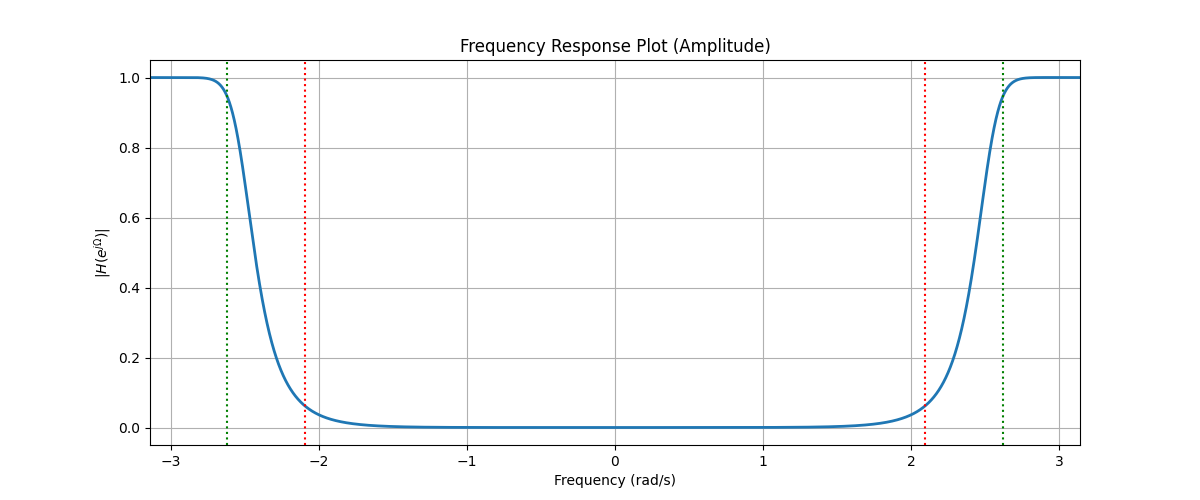
\includegraphics[width=1\linewidth]{frequency_response_amplitude.png}
    \caption{Frequency response plot (from \(-\pi\) to \(+\pi\), amplitude only).}
\end{figure}
In the pass-band region \(\Omega_p=\frac{5\pi}{6}\), we have a near-unity gain. In the stop-band region \(\Omega_s=\frac{2\pi}{3}\), we have strong attenuation.

\section{Design Verification}
\begin{figure}[H]
    \centering
    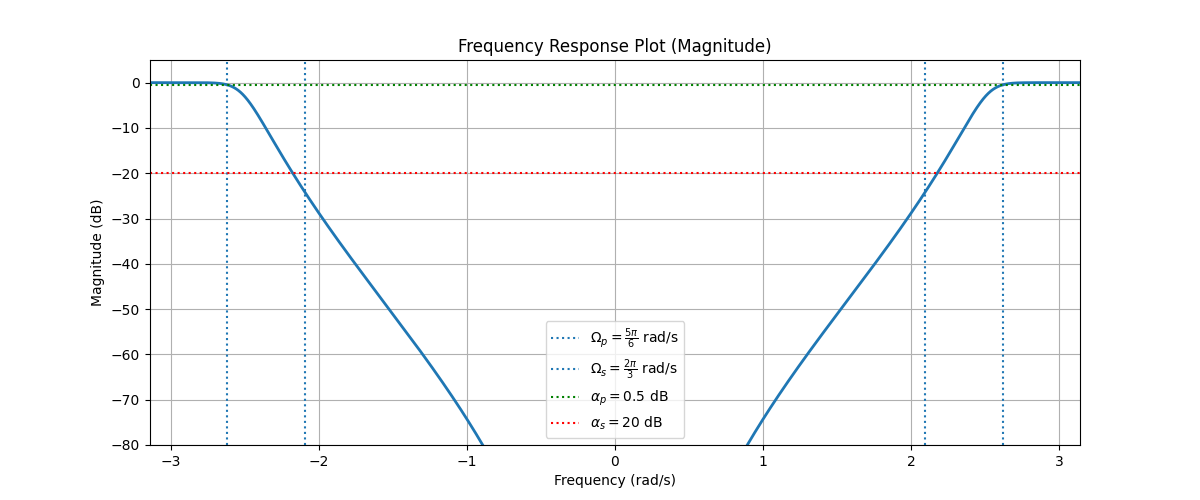
\includegraphics[width=1\linewidth]{frequency_response_magnitude.png}
    \caption{Frequency response plot (from \(-\pi\) to \(+\pi\), magnitude only).}
\end{figure}
We evaluate the frequency response at the pass-band frequency. At \(\Omega_p=\frac{5\pi}{6}\), we find the magnitude to be 0.4978 dB, which is less than the maximum pass-band attenuation of 0.5 dB. At \(\Omega_s=\frac{2\pi}{3}\), we find the magnitude to be 24.2169 dB, which is greater than the minimum stop-band attenuation of 20 dB. Thus, we verify that our design has passed the necessary specifications.


\end{document}
